\section{Tổng quan}
\subsection{Ngôn ngữ lập trình sử dụng: Python}
\subsection{Môi trường hệ điều hành: Windows}

\section{Mô tả chương trình}
\subsection{Chạy phía server}
\subsection{Chạy phía client}
\bf
\begin{enumerate}
\large\item Giao diện
\normalsize
\begin{figure}[H]
\center{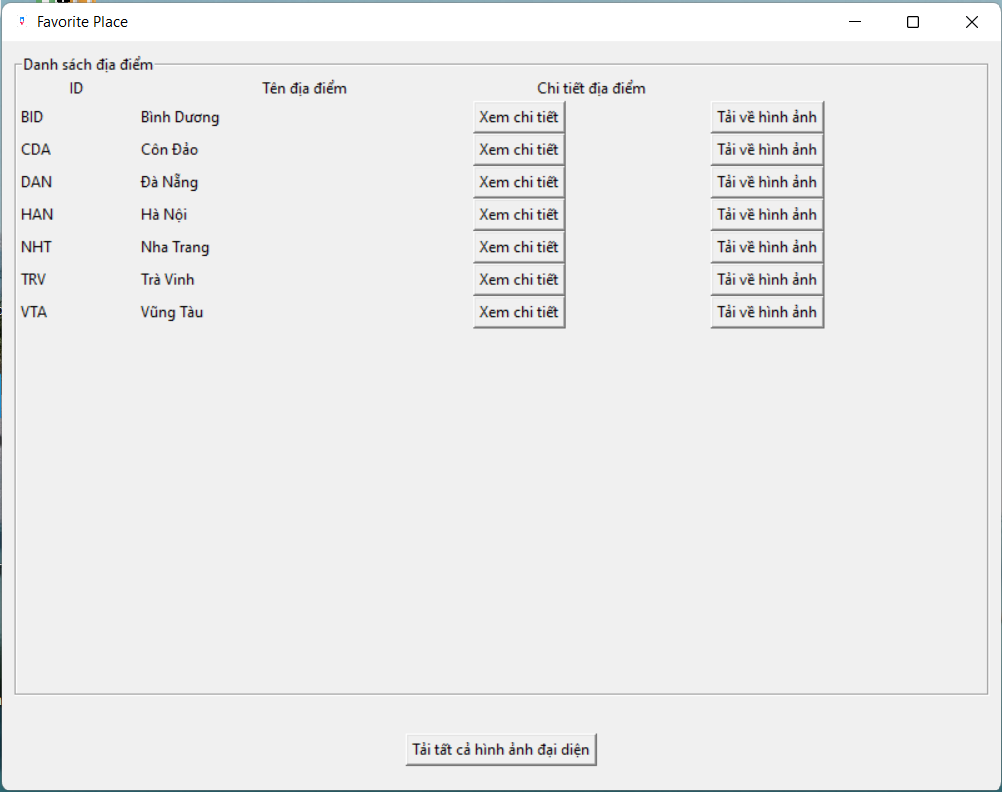
\includegraphics[scale=0.75]{app-description/app}}
\caption{Giao diện phần mềm phía \texttt{client}}
\end{figure}

\large\item Tính năng

\rm
Chương trình cho phép nhiều clients cùng kết nối với server cùng một lúc.

\begin{figure}[H]
\center{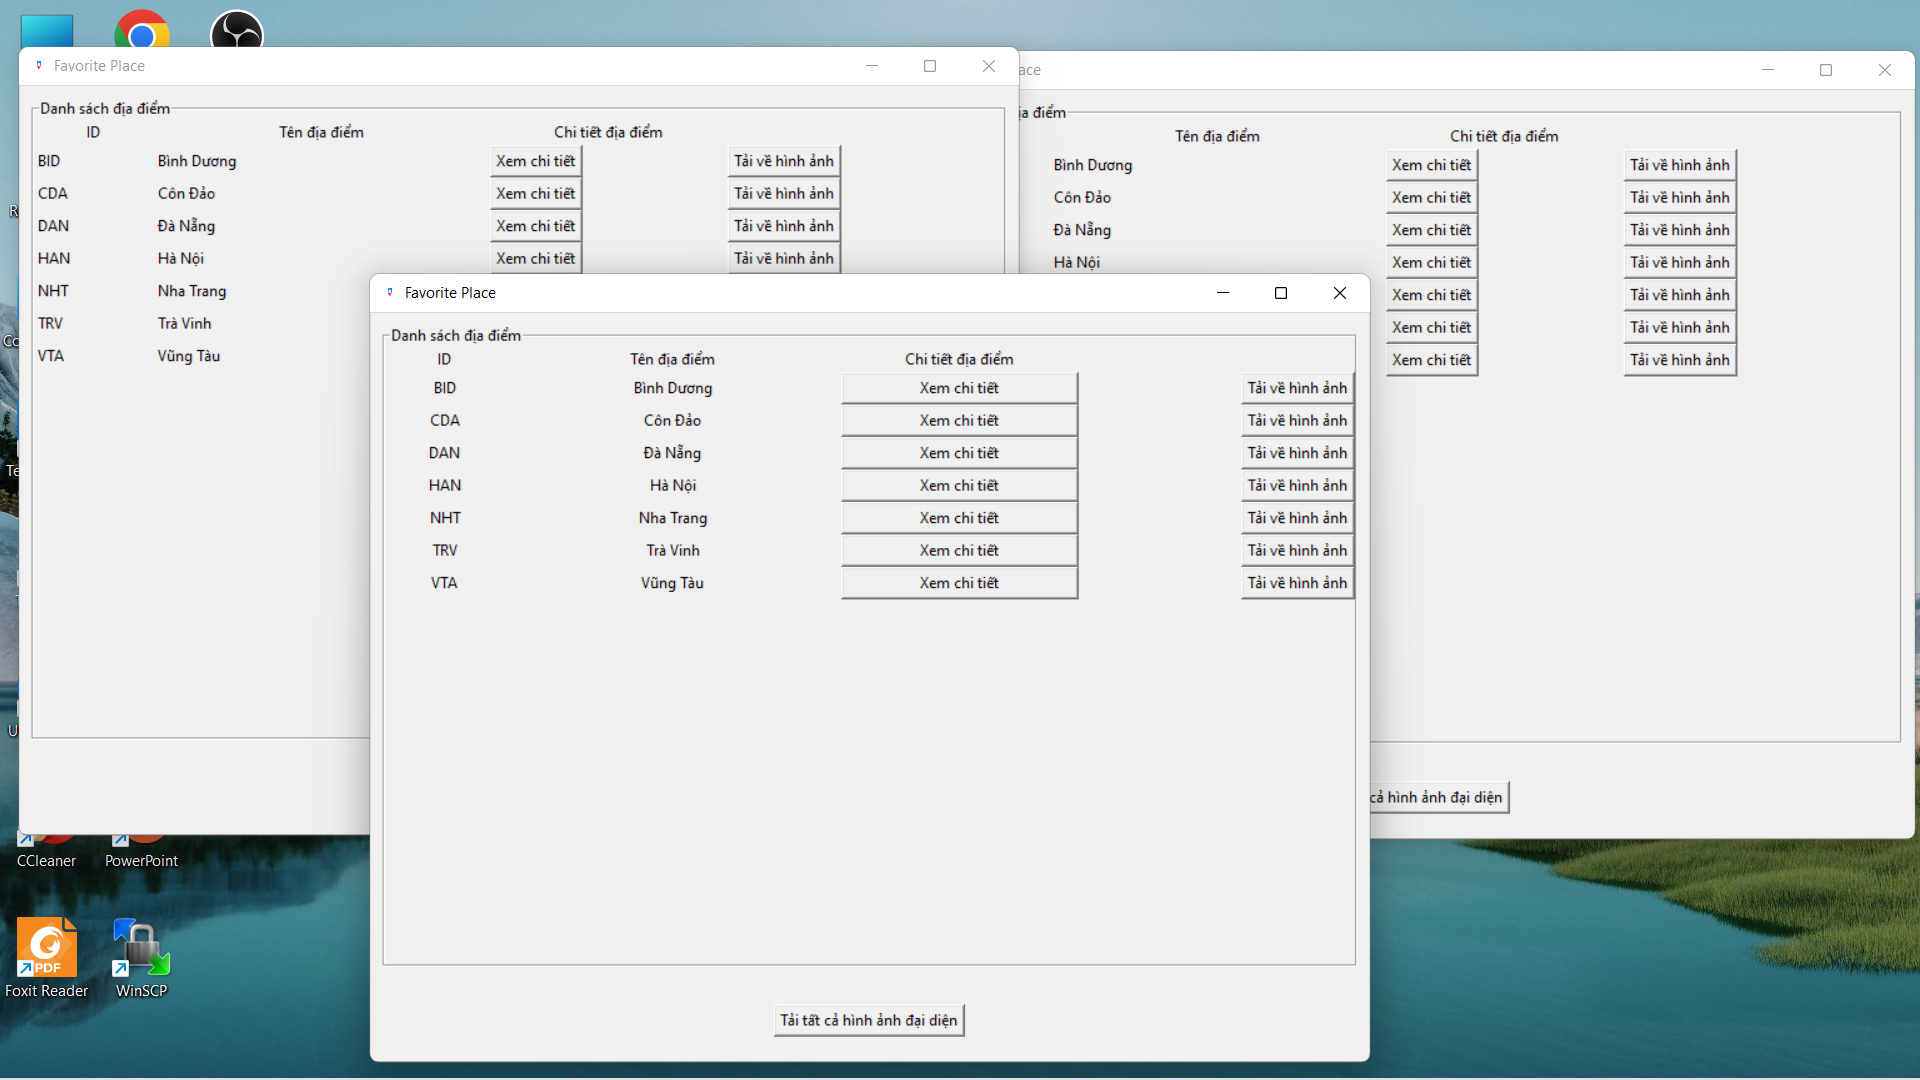
\includegraphics[scale=0.4]{app-description/multi-clients}}
\caption{Cho phép nhiều clients cùng kết nối với server tại một thời điểm}
\end{figure}

\normalsize\bf
\begin{enumerate}
\item \textit{Truy vấn chi tiết thông tin địa điểm}
\rm

Để xem thông tin chi tiết của địa điểm, người dùng click vào thẻ \texttt{Xem chi tiết} trên phần giao diện ứng với địa điểm tương ứng. Màn hình sẽ hiện ra một cửa sổ mới chứa thông tin địa điểm truy vấn, bao gồm tên, tọa độ trung tâm, mô tả ngắn và hình ảnh đại diện của địa điểm đó.

\begin{figure}[H]
\center{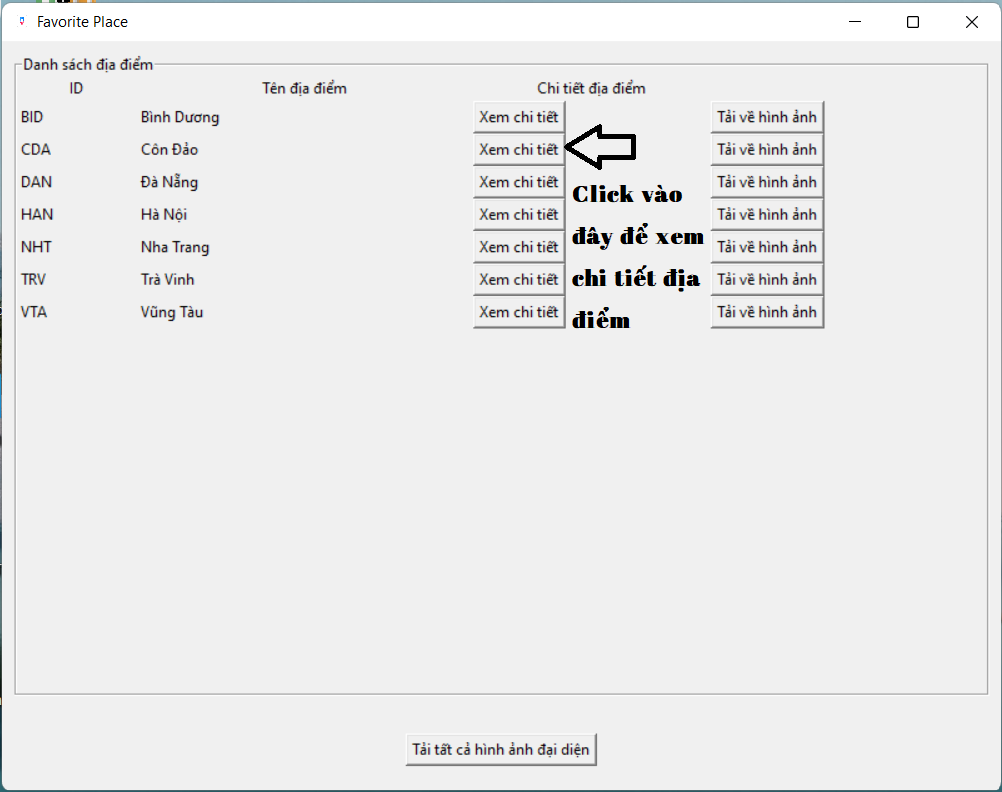
\includegraphics[scale=0.6]{app-description/app-1}}
\end{figure}
\begin{figure}[H]
\center{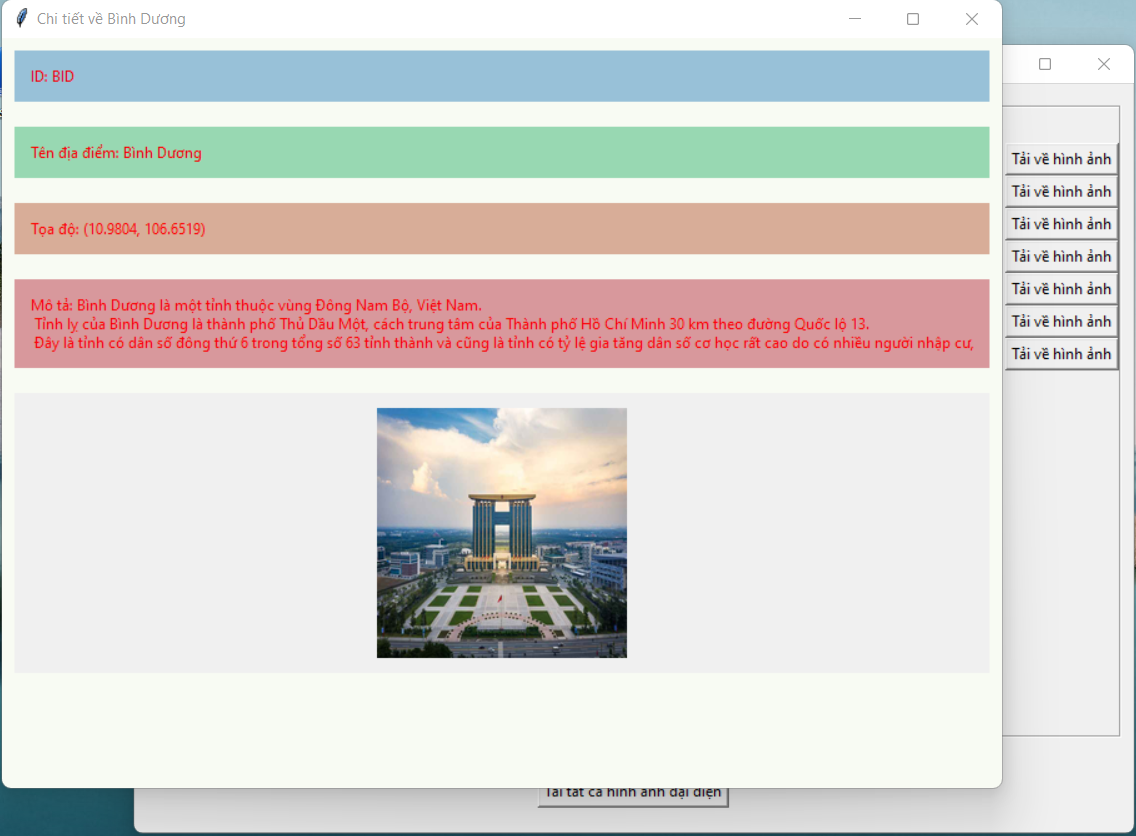
\includegraphics[scale=0.6]{app-description/give-detail-query}}
\caption{Xem thông tin chi tiết tại một địa điểm (Ví dụ: Bình Dương)}
\end{figure}

\bf
\item \textit{Tải về tất cả hình ảnh của một địa điểm}
\rm

Để tải về tất cả hình ảnh của một địa điểm, người dùng click vào thẻ \texttt{Tải về hình ảnh} trên phần giao diện ứng với địa điểm tương ứng. Màn hình sẽ hiện ra một cửa sổ mới chứa các hình ảnh của địa điểm truy vấn, và các hình ảnh được tải về được lưu trong đường dẫn có thể truy cập được.

\begin{figure}[H]
\center{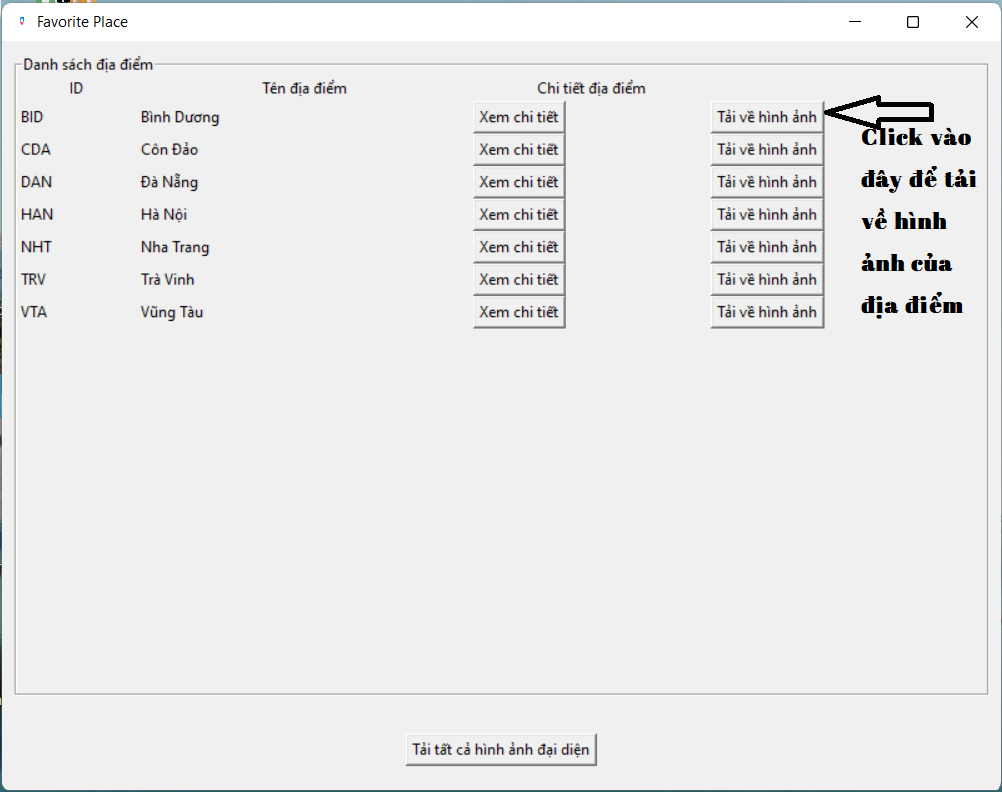
\includegraphics[scale=0.6]{app-description/app-2}}
\end{figure}
\begin{figure}[H]
\center{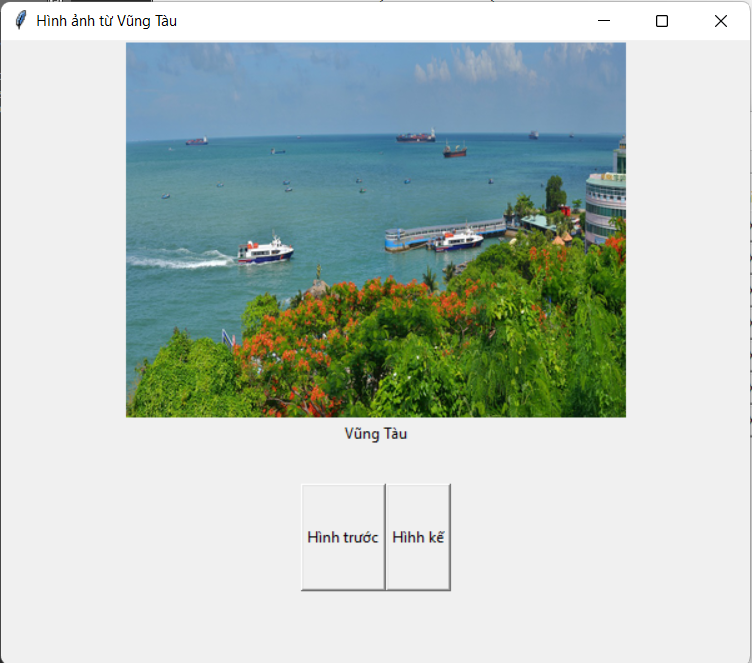
\includegraphics[scale=0.5]{app-description/get-img-1-des-1}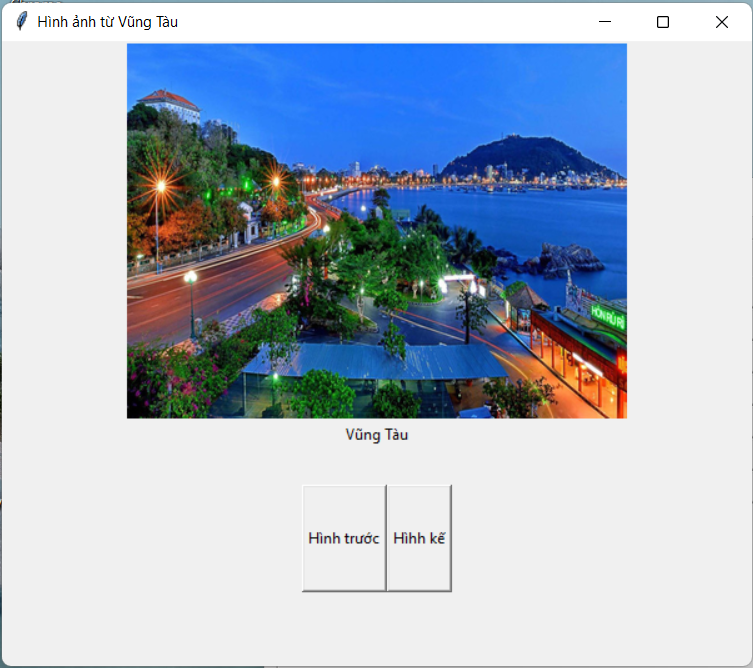
\includegraphics[scale=0.5]{app-description/get-img-1-des-2}}
\caption{Tải về tất cả hình ảnh của một địa điểm}
\end{figure}

\bf
\item \textit{Tải về hình ảnh đại diện của tất cả các địa điểm}
\rm

Để tải về tất cả hình ảnh đại diện của tất cả các địa điểm, người dùng click vào thẻ \texttt{Tải tất cả hình ảnh đại diện} trên phần giao diện. Màn hình sẽ hiện ra một cửa sổ mới chứa các hình ảnh đại diện của tất cả các địa điểm, và các hình ảnh được tải về được lưu trong đường dẫn có thể truy cập được.

\begin{figure}[H]
\center{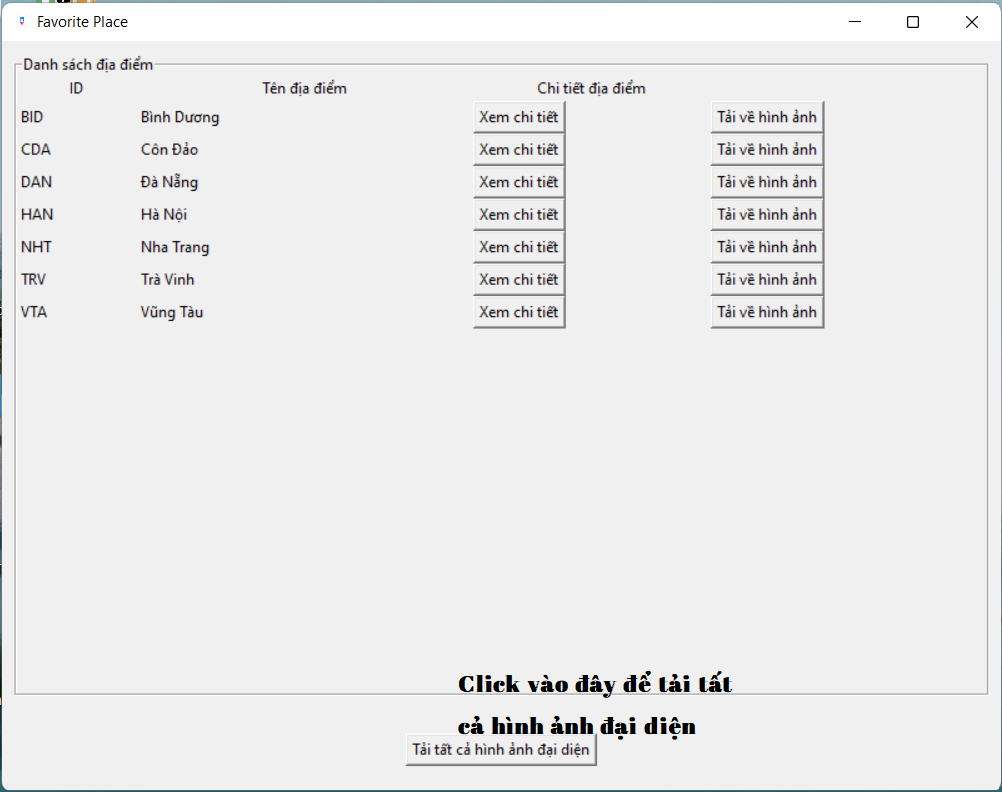
\includegraphics[scale=0.6]{app-description/app-3}}
\end{figure}
\begin{figure}[H]
\center{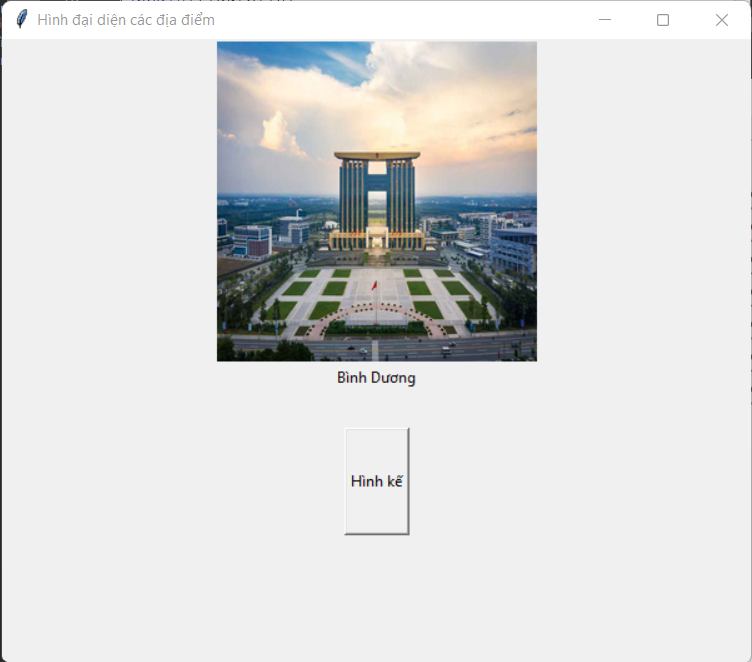
\includegraphics[scale=0.5]{app-description/get-all-avt-1}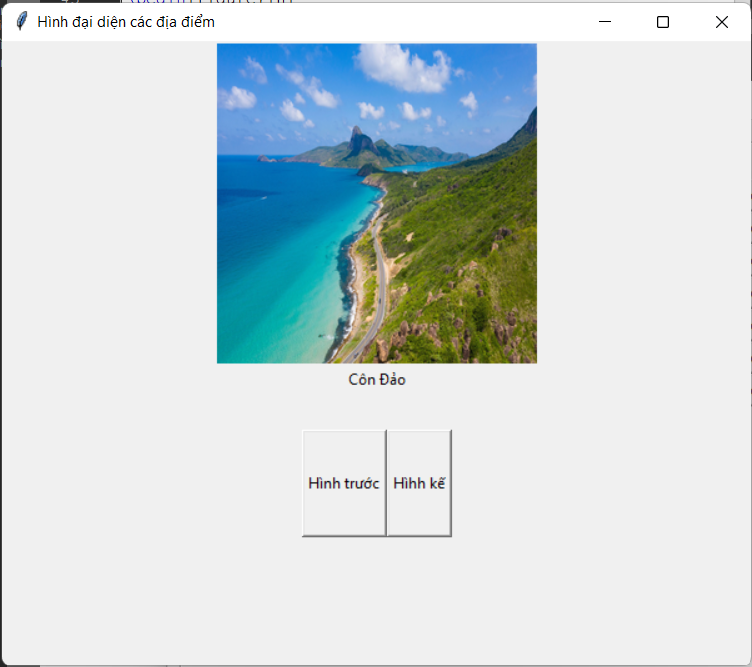
\includegraphics[scale=0.5]{app-description/get-all-avt-2}}
\caption{Tải về hình ảnh đại diện của tất cả địa điểm}
\end{figure}

\end{enumerate}
\end{enumerate}
\rm

